\newpage
\section{So sánh các biến thể của CLIP}

\paragraph{}{CLIP được huấn luyện với nhiều kiến trúc Image Encoder và kích thước khác nhau, dẫn đến các biến thể với hiệu suất và chi phí tính toán khác nhau.}

\begin{figure}[H]
    \centering
    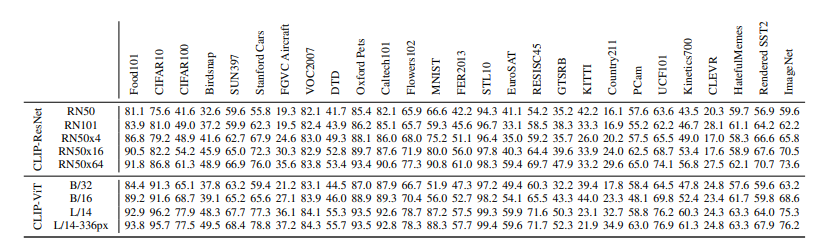
\includegraphics[width=1\linewidth]{img/04-Compare_CLIP.png}
    \caption{Bảng so sánh hiệu suất Zero-shot của các biến thể CLIP trên 17 tập dữ liệu}
\end{figure}

\paragraph{}{Dựa vào bảng so sánh trên, ta có các nhận xét:}
\begin{itemize}
    \item Scaling Laws: Hiệu suất của CLIP tăng lên đáng kể khi tăng kích thước mô hình (cả Image Encoder và Text Encoder) và lượng dữ liệu huấn luyện.
    \item ViT vs. ResNet: Các mô hình Vision Transformer (ViT) thường cho hiệu suất tốt hơn so với các mô hình ResNet có cùng lượng tính toán, đặc biệt là ở quy mô lớn.
    \item Zero-Shot Power: Ngay cả các biến thể nhỏ hơn của CLIP cũng cho thấy khả năng zero-shot ấn tượng trên nhiều bộ dữ liệu và tác vụ khác nhau, vượt xa các phương pháp trước đó.
    \item Tính toán và bộ nhớ: Các mô hình lớn hơn (như ViT-L/14) đòi hỏi tài nguyên tính toán và bộ nhớ GPU đáng kể cho cả huấn luyện và suy luận.
\end{itemize}

\section{Ưu điểm, thách thức}
\paragraph{Ưu điểm nổi bật}{
\begin{itemize}
    \item \textbf{Khả năng Zero-Shot mạnh mẽ:} Đây là đóng góp quan trọng nhất, cho phép áp dụng vào nhiều tác vụ thị giác mà không cần huấn luyện lại hoặc fine-tuning.
    \item \textbf{Học từ dữ liệu web tự nhiên:} Giảm sự phụ thuộc vào các bộ dữ liệu được gán nhãn thủ công tốn kém.
    \item \textbf{Tính linh hoạt cao:} Dễ dàng thích ứng với các tác vụ mới chỉ bằng cách thay đổi mô tả văn bản (prompt engineering).
    \item \textbf{Mô hình nền tảng (Foundation Model):} Có thể được sử dụng làm cơ sở cho nhiều ứng dụng downstream phức tạp hơn (ví dụ: tạo ảnh từ văn bản, VQA).
    \item \textbf{Robustness:} Hiệu suất tốt trên nhiều loại dữ liệu và phân phối khác nhau so với các mô hình chỉ học trên tập dữ liệu cố định.
\end{itemize}
}

\paragraph{Thách thức, hạn chế:}{
\begin{itemize}
    \item \textbf{Khó khăn với tác vụ chi tiết:} CLIP có thể gặp khó khăn với các tác vụ đòi hỏi sự hiểu biết rất chi tiết, ví dụ như đếm số lượng đối tượng nhỏ, nhận diện chữ rất nhỏ (fine-grained OCR), hoặc các mối quan hệ không gian phức tạp.
    \item \textbf{Chi phí tính toán:} Huấn luyện CLIP đòi hỏi tài nguyên tính toán rất lớn. Các mô hình lớn nhất cũng tốn kém khi suy luận.
    \item \textbf{Độ nhạy với Prompt Engineering:} Hiệu suất có thể thay đổi đáng kể tùy thuộc vào cách diễn đạt câu truy vấn văn bản.
    \item \textbf{Dữ liệu "nhiễu" và thiên kiến (Bias):} Vì học từ dữ liệu web, CLIP có thể kế thừa các thiên kiến xã hội tiềm ẩn trong dữ liệu đó.
    \item \textbf{Không phải là "All-in-one":} Mặc dù mạnh mẽ, CLIP không phải lúc nào cũng là lựa chọn tốt nhất cho mọi tác vụ thị giác. Các mô hình chuyên biệt được huấn luyện có giám sát vẫn có thể vượt trội trong các lĩnh vực hẹp cụ thể.
    \item \textbf{Khả năng trừu tượng hóa hạn chế:} Gặp khó khăn khi khái quát hóa với các khái niệm hoàn toàn mới hoặc trừu tượng mà không có sự tương đồng trong dữ liệu huấn luyện
\end{itemize}
}